%!TEX encoding = UTF-8 

\chapter{Proposed Architecture}
\label{chap:proposed_architecture}

In \ac{RobotCub}\index{RobotCub} and in this thesis project too, manipulation is seen as a means to assist perception\index{perception} under uncertainty. Often, vision alone is not enough to reliably segment\index{image segmentation} distinct objects from the background. Overlapping objects or similarity in appearance to the background can confuse many visual segmentation algorithms. Rather than defining an object in terms of its appearance or shape as a predefined model, we propose a simple framework, where only the position and orientation of a tracked object are taken into consideration. This will be done by \emph{estimating the orientation as the major axis of the best-fit enclosing ellipse\index{ellipse} that surrounds the object}.

In this section we will describe the proposed visual processing (a segmentation based on colour histograms), our 3D reconstruction technique, and the applications to object manipulation tasks.

%%%%%%%%%%%%%%
%%%%%%%%%%%%%%
\section{Visual Processing}

Using \ac{CV} to control grasping tasks is natural, since it allows to recognize and to locate objects~\cite{dufournaud:1998}. In particular, stereopsis can help robots reconstruct a 3D scene and perform visual servoing.

As discussed in Section~\ref{sec:segmentation}, the problems of object tracking and image segmentation can be handled from several different perspectives. There exist elaborate methods which implement tracking, based, for example, on: contour tracking by the means of \emph{snakes}; association techniques and matrix Eigenvalues (Eigenspace matching); maintaining large sets of statistical hypotheses; computing a convolution of the image with predefined feature detector patterns. Most of these techniques, though, are computationally expensive and not suited for our framework, which must be simple enough and be able to run in real time, such as at 30 \ac{FPS}.

So, \ac{CV} algorithms that are intended to form part of a \ac{PUI}, such as our problem and all \ac{RobotCub} research in general, must be fast and efficient. They must be able to \emph{track in real time}, yet not absorb a major share of the computational resources that humanoid robots have.

The majority of the available segmentation algorithms in literature do not cover all the needs of our objective optimally, because they do not possess all of our requirements:
\begin{itemize}
\item being able to track similar objects;

\item being robust to noise;

\item working well and reasonably \emph{fast}, since the tracking algorithm is going to be run in parallel with a considerable set of computationally heavy tasks, so that the robot arm is able to intercept and grasp objects;

\item in particular, we want to run several concurrent instances of the algorithm at the same time, so performance is an important requirement.
\end{itemize}

\bigskip

A possible approach we initially thought of was to interpret motion statistically: by performing a Bayesian interpretation of the problem, the solution of motion estimation could be translated to inferring and comparing different similarity functions, generated from different motion models.

Alternatively, we could have used the \ac{EM}\index{image segmentation!clustering!EM} algorithm\footnote{A variant of $k$-Means (see Section~\ref{kmeans}).} to choose the best model. This method is frequently employed in statistical problems, and it consists of two phases, shown in~Algorithm~\ref{algo:em}.

\begin{algorithm}
\caption{\acl{EM} (\acs{EM})}
\label{algo:em}
\begin{algorithmic}[1]
\STATE (E step) Extrapolate a parameterized likelihood.
\STATE (M step) Maximize the expected likelihood found in the E step.
\end{algorithmic}
\end{algorithm}

More precisely, in the E step we associate all the points that correspond to a randomly chosen model, and in the M step we update the model parameters basing on the points that were assigned to it. The algorithm is iterated over and over, until the model parameters converge.

The solutions recalled so far in this chapter deal with a problem that is similar to the one we want to address---on the one hand, we need to establish \emph{a~priori} the set of motion models that the object can present; on the other hand we wish to choose the best possible motion model.

\bigskip

To sum up, several different approaches for segmentation are possible; though, since the development of a tracking algorithm is not the main objective of this work (it is but an initial component of it), and performance is a strong requirement, we opted for using a simple, ready-made solution from OpenCV\index{OpenCV} (Intel Open Source Computer Vision Library,~\cite{link:opencv}), which is a library of C/C++ functions and algorithms frequently used in image processing. The method that we chose was \ac{CAMSHIFT}\index{CAMSHIFT}, detailed further down. However, some custom modifications were applied by us on the OpenCV version of \ac{CAMSHIFT}. The most relevant of them are these two: 
\begin{itemize}
\item we compute the enclosing ellipse\index{ellipse} of an object by focusing the attention on the axes and centroid of such an ellipse (rather than memorizing and transmitting a whole rectangular area, we just handle, for instance, the major axis of the ellipse);

\item we add networking capabilities to the OpenCV implementation of \ac{CAMSHIFT}, by encapsulating it into the \ac{YARP} module system (see Section~\ref{sec:yarp}) and using a middleware\index{middleware} mechanism. This makes it possible to run several instances of the tracker in parallel, for example two trackers to track an object with stereopsis\index{stereopsis}, or multiple objects.
\end{itemize}

%%%%%%%%%%%%%%%
\section{\acs{CAMSHIFT} Module}
\label{sec:camshift_module}

The \acl{CAMSHIFT} algorithm\index{CAMSHIFT}, or \acs{CAMSHIFT} for short, is based on Mean~Shift~\cite{comaniciu:1997}, which in turn is a robust, non-parametric iterative technique for finding the mode of probability distributions. Interestingly, the Mean Shift algorithm was not originally intended to be used for tracking, but it proved effective in this role nonetheless (see~\cite{bradski:1998}).

\ac{CAMSHIFT} is fast and simple; as such, it fulfils the requirements of our project. It is a technique based on colour, however, contrary to similar algorithms, \ac{CAMSHIFT} does \emph{not} take into account colour correlation, blob growing, region growing, contour considerations, Kalman filter smoothing and prediction (all of which are characteristics that would place a heavy burden on computational complexity and speed of execution).

The complexity of most colour-based tracking algorithms (other than \ac{CAMSHIFT}) derives from their attempt to deal with \emph{irregular object motion}, which can be due to:
\begin{itemize}
\item perspective\index{perception} (near objects to the camera seem to move faster than distal ones);

\item image noise;

\item distractors, such as other shapes present in the video scene;

\item occlusion\index{occlusion} by hands or other objects;

\item lighting variation.
\end{itemize}

Indeed, all of the above are serious problems that are worth studying and being modelled for certain practical applications, however the main trait of \ac{CAMSHIFT} is that it is a fast, computationally-efficient algorithms that mitigates those issues ``for free'', i.e., during the course of its own execution.

\bigskip

\begin{algorithm}
\caption{Mean Shift}
\label{algo:meanshift} \index{Mean Shift}
\begin{algorithmic}[1]
\STATE Choose a search window size.
\STATE Choose the initial location of the search window.
\STATE Compute the mean location in the search window.
\STATE Centre the search window at the mean location computed in step 3.
\STATE Repeat steps 3 and 4 until convergence (or until the mean location moves less than a preset threshold).
\end{algorithmic}
\end{algorithm}

At the beginning of this section, we mentioned that in general Mean Shift~(see Algorithm~\ref{algo:meanshift}) operates on probability distributions. Therefore, in order to track coloured objects in a video frame sequence, the colour image data has to be represented as a probability distribution~\cite{comaniciu:1997} --- to do this, \emph{colour histograms} are used.

Colour distributions that are derived from video image sequences may change over time, so the Mean Shift algorithm must be modified to dynamically adapt to the probability distribution that it is tracking at a given moment. It is here that the new, modified algorithm --\ac{CAMSHIFT}-- bridges the gap (also see~\ref{img:colour_obj_tracking}).

\bigskip

Given a colour image and a colour histogram, the image produced from the original colour image by using the histogram as a lookup table is called \emph{back-projection image}. If the histogram is a model density distribution, then the back-projection image is a probability distribution of the model in the colour image. \acs{CAMSHIFT}\index{CAMSHIFT} detects the mode in the probability distribution image by applying Mean Shift while dynamically adjusting the parameters of the target distribution. In a single image, the process is iterated until convergence---or until an upper bound on the number of iterations is reached.

A detection algorithm can be applied to successive frames of a video sequence to track a single target. The search area can be restricted around the last known position of the target, resulting in possibly large computational savings. This type of scheme introduces a feedback loop, in which the result of the detection is used as input to the next detection process. The version of \ac{CAMSHIFT} applying these concepts to tracking of a single target in a video stream is called Coupled \ac{CAMSHIFT}\index{CAMSHIFT!Coupled CAMSHIFT}.

The Coupled \ac{CAMSHIFT} algorithm as described in~\cite{bradski:1998} is demonstrated in a real-time head tracking application, which is part of the Intel OpenCV library~\cite{link:opencv}\index{OpenCV}. 

\begin{figure}
\centering
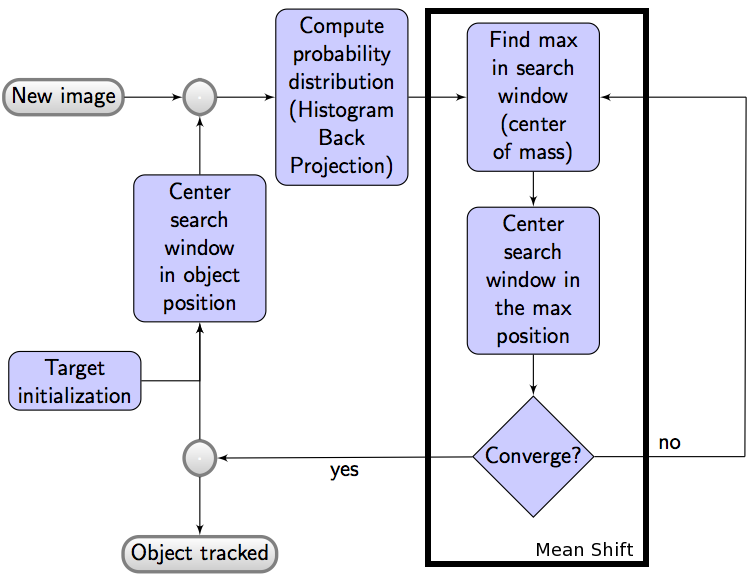
\includegraphics[scale=0.4]{figures/camshift_diag2}
\caption[Block diagram of \acs{CAMSHIFT}]{Block diagram of \ac{CAMSHIFT}.}
\label{img:camshift_diag2}
\end{figure}

% we added computation of major axis of ellipse
% use the 2 extremities as an input for other modules

%%%%%%%%%%%%%%%%%%%%%%%%%%%%%%%%%
\subsection{\acs{CAMSHIFT} and \acs{HSV} Conversion}
\index{HSV}

In order to use a histogram-based method to track coloured objects in a video scene, a probability distribution image of the desired colour present in the video sequence must first be created. For this, one first creates a model of the desired \emph{hue} by using a colour histogram.

The reason why \ac{HSV} space is better suited for our proposed perceptual interface is the following. Other colour models like \ac{RGB}, \ac{CMY}, and YIQ are hardware-oriented~\cite[p.~590]{foley}. By contrast, Smith's \ac{HSV}~\cite{smith:1978} is user-oriented, being based on the intuitive, ``artistic'' approach of tint, shade and tone.

In general, the coordinate system of \ac{HSV} is cylindrical; however, the subset of space within which the model is defined is a hexcone\footnote{Six-sided pyramid.}, as in Fig.~\ref{fig:hsv}. The hexcone model is intended to capture the common notions of hue, saturation and value:
\begin{itemize}
\item Hue is the hexcone dimension with points on it normally called red, yellow, blue-green, etc.;

\item Saturation measures the departure of a hue from achromatic, i.e., from white or gray;

\item Value measures the departure of a hue from black (the colour or zero energy).
\end{itemize}
These three terms are meant to represent the artistic ideas of hue: tint, shade and tone.

The top of the hexcone in Fig.~\ref{fig:hsv} corresponds to $V = 1$, which contains the relatively bright colours. Descending the V axis gives smaller hexcones, that correspond to smaller (darker) \ac{RGB} subcubes in Fig.~\ref{fig:rgb}.

%The colours of the $V = 1$ plane are not all of the same perceived brightness, however: colour plates II.7 and II.8 show the colour model.

\begin{figure}
\centering
\subfloat[][RGB colour cube.]
{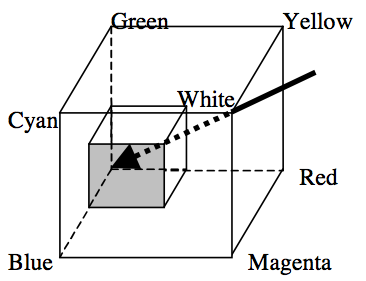
\includegraphics[width=.45\columnwidth]{figures/rgb} \label{fig:rgb} } \quad
% %necessary to prevent line break
\subfloat[][HSV colour system.]
{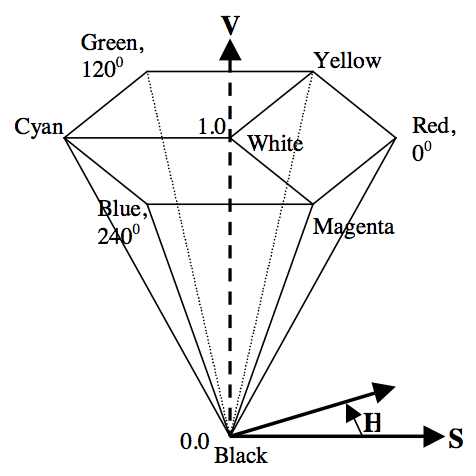
\includegraphics[width=.45\columnwidth]{figures/hsv} \label{fig:hsv} }

\caption[RGB and HSV colour spaces]{RGB and HSV colour spaces. In the single-hexcone HSV model, the $V = 1$ plane contains the RGB model's $R = 1, G = 1$, and $B = 1$ planes in the regions shown.}
\label{fig:rgb-hsv}
\end{figure}

The \ac{HSV} colour space is particularly apt to capture senses and perception, more so than \ac{RGB}. \ac{HSV} corresponds to projecting standard Red, Green, Blue colour space along its principle diagonal from white to black \cite{smith:1978}, as seen looking at the arrow in Fig.~\ref{fig:rgb}. As a result, we obtain the hexcone in Fig.~\ref{fig:hsv}. 
\ac{HSV} space separates out Hue (colour) from Saturation (i.e., how concentrated the colour is) and from brightness. In the case of \ac{CAMSHIFT}, we create our colour models by taking 1D histograms (with 16 bins) from the H channel in \ac{HSV} space.


% check:
% ignore (?) Hue component => invariant to colour
% ignore (?) Intensity component => invariant to illumination

\ac{CAMSHIFT}\index{CAMSHIFT} is designed for dynamically-changing distributions. These occur when objects in video sequences are being tracked and the object moves so that the size and location of the probability distribution changes in time. The \ac{CAMSHIFT} algorithm adjusts the search window size in the course of its operation. Instead of a set or externally adapted window size, \ac{CAMSHIFT} relies on the zeroth moment information, extracted as part of the internal workings of the algorithm, to \emph{continuously} adapt its window size within or over each video frame.

The zeroth moment can be thought of as the distribution ``area'' found under the search window~\cite{bradski:1998}. Thus, window radius, or height and width, is set to a function of the zeroth moment found during search. \ac{CAMSHIFT}, outlined in Algorithm~\ref{algo:camshift}, is then calculated using any initial non-zero window size. 

\begin{algorithm}
\caption{\acs{CAMSHIFT}}
\label{algo:camshift}
\begin{algorithmic}[1]
\STATE Choose the initial location of the search window.
\STATE Perform Mean Shift as in Algorithm~\ref{algo:meanshift}, one or more times. Store the zeroth moment.
\STATE Set the search window size equal to a function of the zeroth moment found in Step~2.
\STATE Repeat Steps~2 and~3 until convergence (mean location moves less than a preset threshold). 
\end{algorithmic}
\end{algorithm}


%%%%%%%%%%%%%%%%%%%%%%%%%%
%%%%%%%%%%%%%%%%%%%%%%%%%%
\section{3D Reconstruction Approach}
\label{sec:3d_recon_approach}\index{3D reconstruction}

In order for a humanoid robot to be able to do things in the world, it requires to have a tridimensional perception, which is what we want to accomplish in this module, in a precise yet simple and efficient (fast) way.

The anthropomorphic head of Baltazar (Fig.~\ref{img:balta_head_real}, p.~\pageref{img:balta_head_real}) has two cameras, mounted in a way similar to the eyes of a human being (Fig.~\ref{fig:balta_cam}, p.~\pageref{fig:balta_cam}).

The notion of \emph{depth} is thus obtained from the combination of information that comes from the two cameras. In this section, we will explain a method to determine the coordinates of one point in the area that is visible from both cameras at a given moment. In particular, we want to reconstruct the 3D coordinates of two points for each object, corresponding to the two extremities of the major axis of the best-fit ellipse to the object. This visual simplification facilitates real-time performances and at the same time it opens the way for manipulation tasks.

%\bigskip

%%%%%%%%%%%%%%%%%%%%%%%%%%%%%%%%
\subsection{From Frame Coordinates to Image Coordinates}

A digitalized image is usually stored in a framebuffer which can be seen as a matrix of pixels with $W$ columns (from ``width'') and $H$ rows (from ``height'').

\begin{figure}
\centering
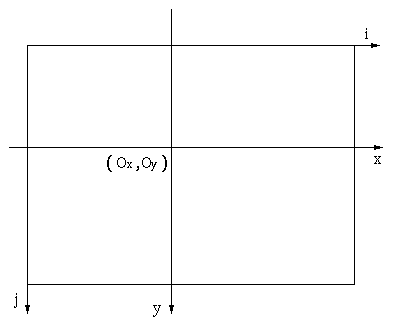
\includegraphics[scale=0.55]{figures/image_coords}
\caption[Image coordinates]{Image coordinates.}
\label{img:image_coords}
\end{figure}

Let $(i,j)$ be the discrete frame coordinates of the image with origin in the upper-left corner, $(O_x,O_y)$ be the focal point of the lens (the intersection between the optical axes and the image plane) in the frame coordinates, and $(x,y)$ be the image coordinates, as illustrated in Fig~\ref{img:image_coords}.

Image coordinates relate to frame coordinates in this way:
\begin{gather}
x = (i - O_x) \cdot S_x \\
y = (j - O_y) \cdot S_y
\end{gather}
where $S_x,S_y$ are the horizontal and vertical distances of two adjacent pixels in the framebuffer.

\bigskip


An \emph{a priori} hypothesis is that we know the relative displacement of the two cameras (rotation and translation) at all times. This makes sense, as we can continuously update the angle values in our software module, receiving instantaneous values from the robot encoders, for example at a frequency of one update per second.

The matrix of intrinsic parameters\index{intrinsic parameters} of a camera, which sets the relationship between a 3D point and the pixels in a sensor, will not be explicitly computed in this project. In other words, we avoid the calibration\index{calibration} phase. The only aspects that we will consider are:
\begin{itemize}
\item image resolution;

\item focal distance\index{focal distance}; and

\item pixel size.
\end{itemize}




% passage from reconstruction to triangulation?
% triangulation:

In stereo analysis\index{stereopsis}, \emph{triangulation}\index{triangulation} is the task of computing the 3D position of points in the images, given the disparity map and the geometry of the stereo setting. The 3D position $(X, Y, Z)$ of a point $\mathbf{P}$ can be reconstructed from the perspective projection\index{perspective projection} (see Fig.~\ref{img:perspective_geom}, p.~\pageref{img:perspective_geom}) of $\mathbf{P}$ on the image planes of the cameras, once the relative position and orientation of the two cameras are known.

For example, if we choose the 3D world reference frame to be the left camera reference system, then the right camera is translated and rotated with respect to the left one, therefore six parameters will describe this transformation.

In the most general case, the right camera can be rotated with respect to the left one (or vice versa) in three directions.


\bigskip

% triangulation.webarchive started here
%%%%%%%%%%%%%%%
%\subsection{Camera Model}

For 3D reconstruction\index{3D reconstruction}, we use a pinhole camera model\index{pinhole camera model} like the one in Fig.~\ref{img:pinhole}.

\begin{figure}
\centering
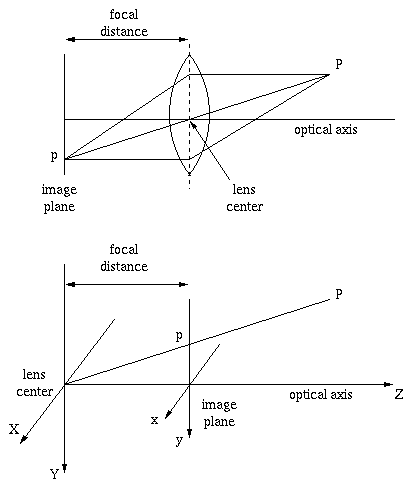
\includegraphics[scale=0.55]{figures/pinhole}
\caption[Pinhole camera model]{Pinhole camera model.}
\label{img:pinhole}
\end{figure}

The relationships that exist between the world coordinates of a point $\mathbf{P} = (X, Y, Z)$ and the coordinates on the image plane $(x, y)$ in a pinhole camera are
%
\begin{gather}
x = F \cdot X / Z \\
y = F \cdot Y / Z
\end{gather}
%
where lower-case letters refer to \emph{image} position, upper-case ones to \emph{world} position (in metres), and $F$ is the focal distance\index{focal distance} of the lens (also in metres).


Considering the two cameras and referring as $B$ to the baseline (distance between the optical centres of them), we can now obtain the missing coordinate $Z$:
%
\begin{gather}
y_L = \frac{F Y_L}{Z_L} \\
Y_R = Y_L - B \\
Z_L = Z_R = Z \\
y_R = \frac{F Y_R}{Z_R} = F \frac{Y_L - B}{Z} \\
y_L - y_R = F \frac{B}{Z} \Longleftrightarrow Z = \frac{F B}{y_L - y_R}.
\end{gather}


We will now analyze the case in which the two cameras are in an arbitrary relative orientation. A description of various vergence\index{vergence} situations can be consulted in~\cite{bernardino:1999}.

\begin{figure}
\centering
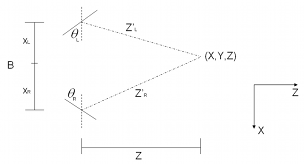
\includegraphics{figures/vergence}
\caption[3D reconstruction scheme]{3D reconstruction scheme for a stereo pair of cameras with arbitrary vergence.}
\label{img:vergence}
\end{figure}

Looking at Fig.~\ref{img:vergence}, we can thus write down the following equations for the $Z$ coordinate:
%
\begin{gather}
\tan (\theta_L + x_L / F) = \frac{B/2}{Z} \\
\tan (\theta_R + x_R / F) = \frac{B/2}{Z} \\
Z = \frac{B}{\tan(x_L / F + \theta_L) - \tan(x_R / F + \theta_R)}.
\end{gather}

As for the $X$ coordinate, we obtain:
%
\begin{gather}
\tan(\theta_L + x_L / F) = \frac{X_L}{Z} \\
\tan(\theta_R + x_R / F) = \frac{X_R}{Z} \\
X = - \frac{Z}{2} \bigl[ \tan(x_L / F + \theta_L) + \tan(x_R / F + \theta_R) \bigr].
\end{gather}

Finally, the 3D reconstructed coordinate $Y$ is obtained like this:
%
\begin{gather}
Z_{R}' = Z / \cos \theta_R \\
Z_{L}' = Z / \cos \theta_L \\
Y = \frac{Z y_R}{2 F \cos \theta_R} + \frac{Z y_L}{2 F \cos \theta_L}
\end{gather}










In order to determine the coordinates of an object in a fixed reference frame, it is necessary to consider the forward kinematics of the head\index{Baltazar!head} of Baltazar (see Section~\ref{sec:balta_head}). From coordinates that are expressed in the image plane, we want to obtain coordinates in a fixed reference frame (a frame attached to the robot torso, which does not move).

Recall the scheme of Baltazar head, illustrated in Fig.~\ref{img:balta_head_scheme}. The expression given in Eq.~\ref{eq:im2fix} was obtained from geometrical analysis, and it provides a relationship between coordinates in the image plane (of one of the two cameras) with the coordinates expressed in a fixed frame.

\begin{equation}\label{eq:im2fix}
{\mathbf{P}}_l = {\mathbf{R}}_l (\mathbf{P} - {\mathbf{t}}_l).
\end{equation}

For the sake of simplicity, Eq.~\ref{eq:im2fix} refers to the left camera case, thus the $l$ subscript. The rotation and translation matrices are, in particular, equal to
%
\begin{equation}
\begin{split}
{\mathbf{R}}_l =	&\begin{bmatrix}
				c_p c_l - c_t s_p s_l	&	- s_p s_t	&	c_t c_l s_p + c_p s_l \\
				- s_t s_l			&	c_t		&	c_l s_t \\
				- c_l s_p - c_p c_t s_l&	- c_p s_t	&	c_p c_t c_l - s_p s_l
				\end{bmatrix}; \\
{\mathbf{t}}_l =		&\begin{bmatrix}
				- B' c_l - t_Y s_t s_l + t_Z (- c_l s_p - c_p c_t s_l) \\
				t_Y c_t - t_Z c_p s_t \\
				t_Y c_l s_t - B' s_l + t_Z (c_p c_t c_l - s_p s_l)
				\end{bmatrix}
\end{split}
\end{equation}
%
where $B' = B/2$ (half the baseline distance).






%%%%%%%%%%%%%%%%%%%
%\subsection{Image Projection Model}
%\subsection{Transformation into World Coordinates}

\index{3D reconstruction}
From a geometrical point of view, the camera sensors mounted on the Baltazar head simply measure \emph{relative positions}; these two cameras are used to calculate the position of objects within their workspace, relative to their optical centre. Thus, a 3D point is mapped onto a two-dimensional space, by the means of its projection on the image plane. It is precisely in this way that we obtain the 2D coordinates of a pair of stereo cameras: the resulting coordinates derive from a 3D point located in the surrounding of Baltazar.






%TODO:
% http://eris.liralab.it/wiki/ICubFowardKinematics_right
%- how Baltazar's head calibration works
%- how we compute world-to-camera(s) matrices
%- perspective (not orthographic) projection
%- optical rays
%- software analysis and design; brief UML (classes)
%- software -> Vectors, ports closing gracefully
%- why multiprocess instead of multithread
%- complexity: where is the bottleneck?
%- drawback: can't track rotationally-symmetric objects
%- how we computed new camera parameters for Dragonfly camera with custom res

%%%%%%%%%%%%%%%%%
\subsection{3D Pose Estimation}
\index{3D reconstruction}

Consider now a \emph{target object} placed in front of the robot; tracking is accomplished by running two \ac{CAMSHIFT}\index{CAMSHIFT} processes. Let points $\{p_1, p_2\}_l^{\mathrm{target}}$ and $\{p_1, p_2\}_r^{\mathrm{target}}$ be the extremities of the major ellipse axis expressed in the 2D coordinate frame of the left and right tracker, respectively\footnote{The same considerations apply for stereo tracking and 3D reconstruction of the robot \emph{hand}, but for the sake of simplicity only the target object case is explained here. From now on, the ``target'' exponent in the notation is therefore omitted.}.

A 3D reconstruction process receives the coordinates of the four points $\{p_1, p_2 \}_{l,r}$ as inputs, along with the instantaneous head joint angle values of the robot, used to compute the time-varying extrinsic camera parameter matrices: not just the target object, but also the robot cameras may be moving during experiments. Transformation matrices $\leftidx{^w}{\mathbf{T}}_l$ and $ \leftidx{^w}{\mathbf{T}}_r$ represent the roto-translations occurring, respectively, from the left and right camera reference frame to the world (torso) reference frame, as shown in Fig.~\ref{img:balta_head_transf}.

\begin{figure}
\centering
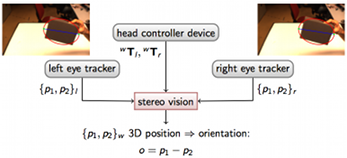
\includegraphics{figures/recon_module}
\caption[3D reconstruction software module scheme]{3D reconstruction software module scheme, outlining the data that are passed as inputs/outpus among \ac{YARP} modules.}
\label{img:recon_module}
\end{figure}

Fig.~\ref{img:recon_module} shows how the 3D reconstruction\index{3D reconstruction} module works. It receives inputs from two \ac{CAMSHIFT}\index{CAMSHIFT} trackers (one per each eye), it receives the instantaneous head joint angles (with which it builds transformation matrices), then finally it computes estimated coordinates and orientation of a tracked object.

Thanks to how \ac{YARP}\index{YARP} is designed, we can easily run various concurrent instances of this modules in parallel. Specifically, in the grasping preparation (visual servoing) phase we will be interested in 3D reconstructing the target object and the robot hand at the same time.

Once the reconstruction is computed, 3D coordinates of $\{ p_1, p_2\}$ are obtained.
The difference vector $p_1 - p_2$ encodes the orientation of the target.


\begin{figure}
\centering
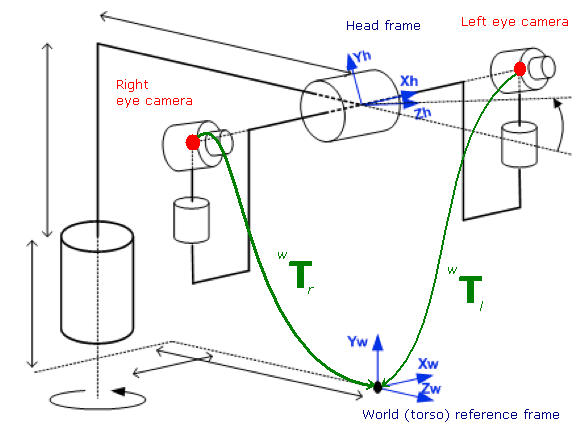
\includegraphics[scale=0.5]{figures/balta_head_transf}
\caption[Structure of Baltazar head with transformation matrices]{Mechanical structure of Baltazar head, its reference frames and points of interest. Transformation matrices are highlighted in green.}
\label{img:balta_head_transf}
\end{figure}












%%%%%%%%%%%%%%%%%%%%%%
\section{Object Manipulation Approaches}
\index{manipulation}

% how we implement concurrency, how we avoid deadlocks and problems
% reaching FSM

% why our algorithms are good


%TODO:
%- object orientation => hand orientation
%- MATLAB simulation of arm to study fw.kin., with studied SDH params

As mentioned in p.~\pageref{intro:reaching_phases}, in this work we consider two distinct phases for a manipulation task:

\begin{description}
\item[reaching preparation:]\index{reaching} this phase aims at bringing the robot hand to the vicinity of the target. It is applied whenever a target is identified in the workplace but the hand is not visible in the cameras. The measured 3D target position is used, in conjunction with the robot arm kinematics, to place the hand close to the target. Inevitably, there are mechanical calibration errors between arm kinematics and camera reference frames, so the actual placement of the hand will be different from the desired one. Therefore, the approach is to command the robot not to the exact position of the target but to a distance safe enough to avoid undesired contact both with the target and the workspace.

\item[grasping preparation:]\index{grasping} in this phase, both target and hand are visible in the camera system and their posture can be obtained by the methods previously described. The goal is now to measure the position and angular error between target and hand, and use a \ac{PBVS} approach to make the hand converge to the target. The features used in such an approach are 3D parameters estimated from image measurements---as opposed to \ac{IBVS}\index{Visual Servoing!Image-Based Visual Servoing}, in which the features are 2D and immediately computed from image data.
\end{description}

Reaching preparation is relatively easy, since in this phase we just position the arm to the vicinity of the target object (within a threshold of 20 cm). The arm starts moving from a predefined position outside of the field of view of the two cameras, and it reaches the position estimated by the inverse kinematics solver.

On the other hand, there are two peculiarities in the presented grasping preparation approach:
%
\begin{itemize}
\item Normally, \ac{PBVS}\index{Visual Servoing!Position-Based Visual Servoing} requires the 3D model of the observed object to be known~\cite{hutchinson:1996}, but in our framework one gets rid of this constraint: by using the stereo reconstruction technique explained above, the only condition to prepare the servoing task is that the \ac{CAMSHIFT} trackers are actually following the desired objects---whose models are \emph{not} known beforehand.

\item Classical \ac{PBVS} applications consider that target and end-effector positions are measured by different means, e.g. target is measured by the camera and end-effector is measured by robot kinematics. This usually leads to problems due to miscalibrations between the two sensory systems. Instead, in this work, target and hand positions are measured by the camera system in the same reference frame, therefore the system is robust to calibration errors.
\end{itemize}

\begin{figure}
\centering
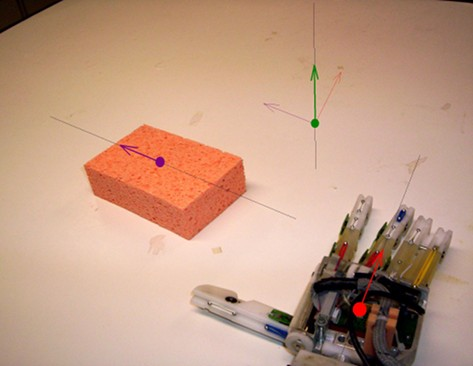
\includegraphics{figures/cross_prod2}
\caption[Cross product between hand and target orientations]{Unit vector of the target object along its orientation axis (purple); unit vector and orientation of robot hand (red); third axis resulting from their cross product, and corresponding unit vector (green).}
\label{img:cross_prod2}
\end{figure}

Having computed 3D position and orientation of both a target object and of the robot hand, features suitable for the application of the \ac{PBVS}\index{Visual Servoing!Position-Based Visual Servoing} technique must be obtained. As described in~\cite{chaumette:visual1}, the robot arm can be controlled by the following law\index{control law}:
%
\begin{equation}\label{eq:cross_prod}
\begin{cases}
\mathbf{v} = -\lambda \left( \left( \mathbf{t}_\textrm{target} - \mathbf{t}_\textrm{hand} \right) + \left[ \mathbf{t}_\textrm{hand}\right]_{\times} \vartheta \mathbf{u} \right)\\
\mathbf{\omega} = -\lambda  \vartheta \mathbf{u}
\end{cases}
\end{equation}
%
where $\mathbf{v}$ and $\mathbf{\omega}$ are the arm linear and angular velocities, $\lambda$ establishes the trajectory convergence time,  $\mathbf{t}_\textrm{target}$ and $\mathbf{t}_\textrm{hand}$ are the target and hand positions, $\left[ \cdot \right]_{\times}$ is the associated skew-symmetric matrix of a vector; $\vartheta, \mathbf{u}$ are the angle-axis representation of the rotation required to align both orientations. Other control laws can be applied to this problem, but they normally rely on an angle--axis parameterization of the rotation.\index{angle--axis parameterization}

It is possible to calculate the required angle $\vartheta$ and axis $\mathbf{u}$ by applying a simple \emph{cross product rule} between the normalized hand and target orientation vectors:
%
\begin{equation}
%\mathbf{u} = o_{\textrm{target}} \times o_{\textrm{hand}} \qquad\textrm{and}\qquad \vartheta = \arcsin \| \mathbf{u} \|_{2}
\begin{cases}
\mathbf{u} = {\mathbf{o}}_{\textrm{target}} \times {\mathbf{o}}_{\textrm{hand}}\\
\vartheta = \arcsin \| \mathbf{u} \|_{2}
\end{cases}
\label{eq:theta_angle}
\end{equation}
%
where $\| \cdot \|_{2}$ is the Euclidean norm, ${\mathbf{o}}_{\textrm{target}}$ is a unit vector in the direction of the target object's reconstructed\index{3D reconstruction} orientation and ${\mathbf{o}}_{\textrm{hand}}$ is a unit vector in the direction of the hand's reconstructed orientation (see Fig.~\ref{img:cross_prod2}).